\nocite{*} %wszystkie wpisy trafią do bibliografii
\lstset{language=Java, tabsize=2,  basicstyle=\footnotesize\ttfamily, keywordstyle=\underbar}

% \setpagenumberingtype{gobble} % Remove page numbers (and reset to 1)
\setcounter{page}{1}
\newgeometry{tmargin=3cm, bmargin=3cm, lmargin=2cm, rmargin=2cm}

\newgeometry{tmargin=3cm, bmargin=3cm, lmargin=2cm, rmargin=2cm}

\thispagestyle {empty}

\begin{center}
	%logo uczelni
	
\includegraphics[scale=0.4]{img/pw}
	
	\vspace{0.5cm}
	
	{\fontsize{20}{20}\selectfont POLITECHNIKA WARSZAWSKA}
	
	\vspace{1.0cm}
	
	\textbf{{\fontsize{14}{14}\selectfont Wydział Mechatroniki}}
	
	\vspace{1.5cm}
	
	\textbf{{\fontsize{14}{14}\selectfont Praca przejściowa}}

	\vspace{2.0cm}
	
	{\fontsize{14}{14}\selectfont Ireneusz Szulc}
	
	\vspace{1cm}
	
	{\fontsize{28}{28}\selectfont Planowanie bezkolizyjnych tras dla zespołu robotów mobilnych}
	
	\vspace{1cm}
	\begin{flushright}
		{\fontsize{14}{14}\selectfont Opiekun pracy: \\ 
		prof. dr hab. Barbara Siemiątkowska}
	
		\vspace{1cm}
		
		% {\fontsize{14}{14}\selectfont Konsultant pracy: \\ 
		% mgr inż. Daniel Koguciuk}
		
	\end{flushright}
	
	\vspace{1cm}
	
	{\fontsize{12}{12}\selectfont Warszawa, 2018}
	
	%\cleardoublepage %nie działa
	
	%\clearpage\mbox{}\clearpage
\end{center}
\clearpage{\pagestyle{empty}\cleardoublepage}
\clearpage

\phantomsection
\addcontentsline{toc}{chapter}{Spis treści}
\tableofcontents
\clearpage

\raggedbottom
% \setpagenumberingtype{arabic} % kontynuowanie numerowania w stylu arabskim

\chapter{Wstęp}
\label{ch:wstep}

\section{Cel pracy}
Przedmiotem niniejszej pracy jest przegląd metod rozwiązujacych zagadnienie planowania bezkolizyjnych tras dla wielu robotów. Stanowi to również wstęp teoretyczny do zaprojektowania algorytmu i implementacji oprogramowania pozwalającego na symulację działania systemu planowania tras.

Praca skupia się na przypadkach, w których mamy do czynienia ze środowiskiem z dużą liczbą przeszkód (np. zamknięty budynek z licznymi ciasnymi korytarzami), gdzie problem blokowania sią agentów prowadzi często do zakleszczenia. Należy wtedy zastosować nieco inne podejścia niż te, które sprawdzają się w przypadku otwartych środowisk, a które zostały opisane np. w pracach: \cite{roszkowska}, \cite{siemiatkowska}
$TODO$ W otwartych środowiskach mogą się dobrze sprawdzić D* albo LRA*

W niniejszej pracy zajmować będziemy się rozwiązaniem problemu, w którym mamy pełną informację o mapie otoczenia oraz o określonym położeniu początkowym i celu dla każdego z robotów. Zadaniem algorytmu będzie wyznaczenie możliwie najkrótszej bezkolizyjnej trasy dla wszystkich robotów. Należy jednak zaznaczyć, że priorytetem jest dotarcie każdego z robotów do celu bez kolizji z innymi robotami, dopiero później chcemy, aby wyznaczone drogi były możliwie najkrótsze.

$TODO$ zagadnienie z robotami holonomicznymi o zajętości przestrzennej równej 1 - nie mogą się mijać w tym samym korytarzu
Założenia pracy:
1. Planowanie tras dotyczy robotów holonomicznych.
2. Metody planowania powinny sprawdzać się w środowiskach z dużą liczbą przeszkód.
Zakres pracy:
1. Przegląd metod i algorytmów wykorzystywanych do koordynacji ruchu robotów.

$TODO$ bedzie to intro przez metody, aby dotrzeć wreszcie do WHCA*

\section{Koordynacja ruchu robotów}
Koordynacja ruchu robotów jest jednym z fundamentalnych problemów w systemach wielu robotów. \cite{optpriorities}

Kooperacyjne znajdowanie tras (ang. Cooperative Pathfinding) jest problemem planowania w układzie wieloagentowym, w którym to agenci mają za zadanie znaleźć bezkolizyjne drogi do swoich, osobnych celów. Planowanie to odbywa się w oparciu o pełną informację o środowisku oraz trasach pozostałych agentów. \cite{cooppath}

$TODO$ RTS - do skrótów
The interest in Multi-Agent Systems (MAS) is getting increased as more
complicated tasks has been introduced that can not be accomplished by a
single agent. Several domains have been built based on MAS, such as Real
Time Strategy (RTS) games 

Problem kooperacyjnego znajdowania tras pojawia się często m.in. w grach komputerowych, gdzie należy wyznaczyć drogi dla wielu jednostek, które mogą blokować się wzajemnie. Algorytmy do wyznaczania bezkolizyjnych tras dla wielu agentów (robotów) mogą znaleźć również zastosowanie w szpitalach (np. roboty TUG i HOMER do dostarczania sprzętu na wyposażeniu szpitala \cite{tughomer}) oraz magazynach (np. roboty transportowe w magazynach firmy Amazon \ref{fig:image_kiva_amazon}).

\begin{figure}[H]
	\centering
	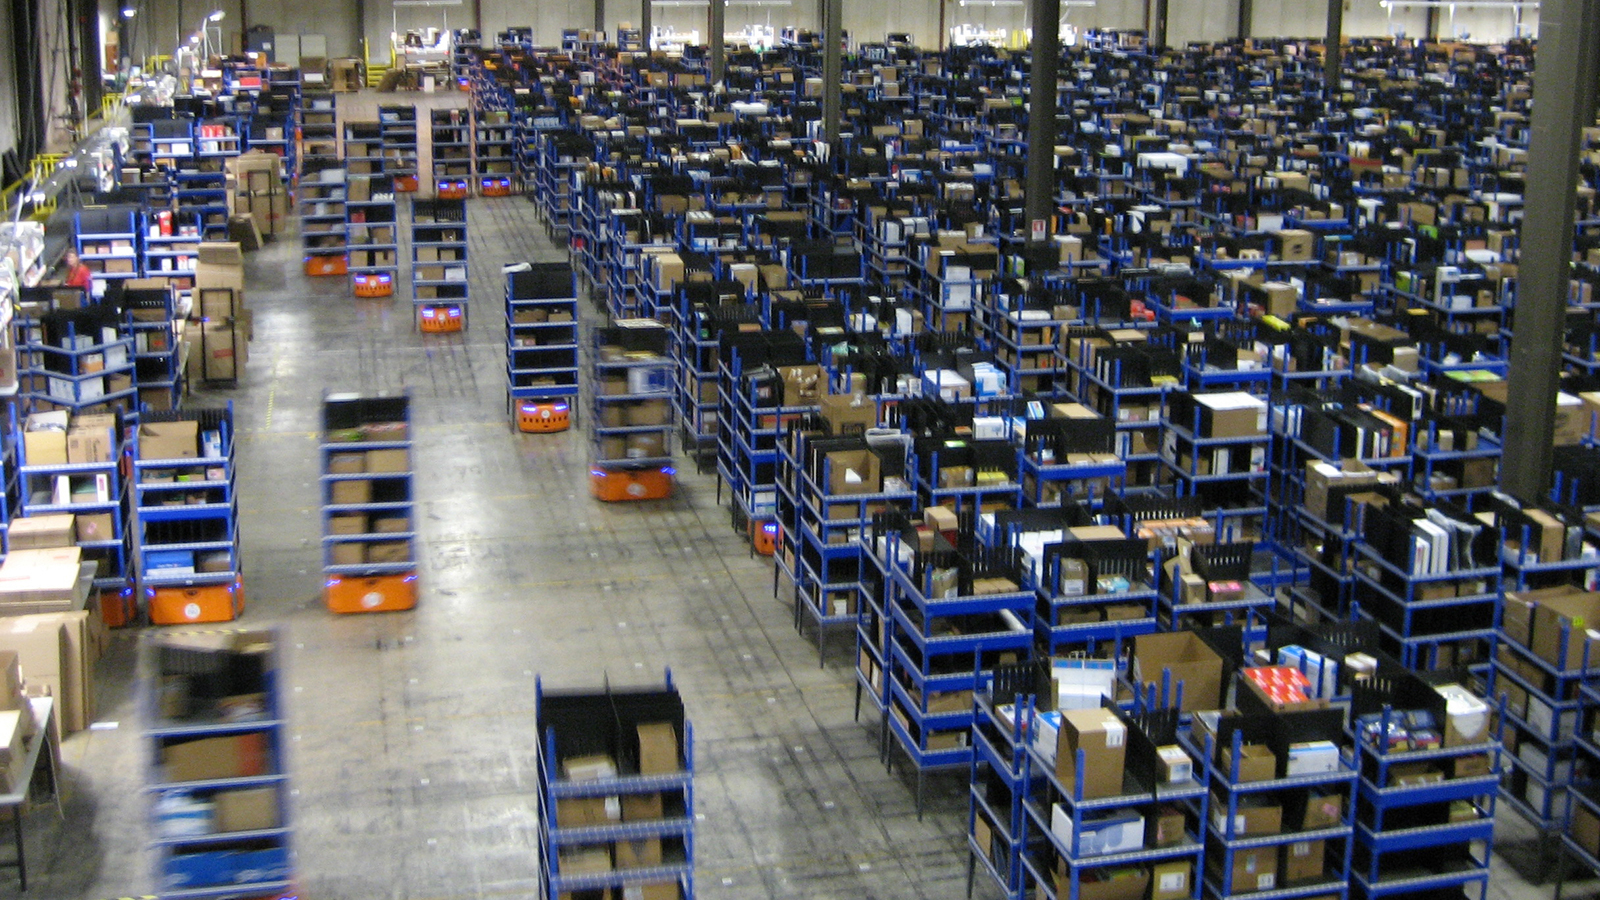
\includegraphics[width=14cm]{img/kiva-amazon}
	\caption{Roboty Kiva pracujące w magazynie firmy Amazon. Źródło: \cite{amazonkiva}}
	\label{fig:image_kiva_amazon}
\end{figure}

\section{Podstawowe pojęcia}
\subsubsection{Przestrzeń konfiguracyjna}
Przestrzeń konfiguracyjna to formalna, matematyczna przestrzeń będąca zbiorem możliwych stanów danego układu fizycznego.
W zależności od rodzaju i liczby wyróżnionych parametrów stanu przestrzenie konfiguracyjne mogą mieć wiele wymiarów.

\subsubsection{Robot holonomiczny}
$TODO$ dopisać definicje i uzupełnić w celu pracy, że będzie to ich dotyczyć

\subsubsection{Metoda hill-climbing}
$TODO$ wyjebać to?
Metoda hill-climbing jest rodzajem matematycznej optymalizacji, lokalną metodą przeszukiwania.
Jest to iteracyjny algorytm, który zaczyna w wybranym rozwiązaniu problemu, następnie próbuje znaleźć lepsze rozwiązanie poprzez przyrostowe zmiany pojedynczych elementów rozwiązania.
Jeśli zmiana przynosi lepsze rozwiązanie, jest wprowadzana do nowego rozwiązania.
Kroki algorytmu powtarzane są dotąd, aż żadne ``udoskonalenie'' nie zostaje znalezione.

\subsubsection{Zupełność algorytmu}
$TODO$

\chapter{Metody planowania tras}
\label{ch:path_planning_methods}

\section{Metody planowania tras}
$TODO$ wyjebać to gówno lub uogólnić
Spośród metod wykorzystywanych do planowania tras dla wielu robotów można wyróżnić dwie zasadnicze grupy \cite{latombe}:
$TODO$ zcentralizowanie nie muszą być optymalne
\begin{itemize}
	\item {\bf Zcentralizowane} - drogi wyznaczane są dla wszystkich agentów na raz (jednocześnie). Metody te potrafią znaleźć wszystkie możliwe rozwiązania (w szczególności to optymalne), ale mają bardzo dużą złożoność obliczeniową ze względu na ogromną przestrzeń przeszukiwania. Z tego powodu stosowane są heurystyki przyspieszające proces obliczania rozwiązania.
	\item {\bf Rozproszone} (ang. {\it decoupled} lub {\it distributed}) - Podejście to dekomponuje zadanie na niezależne lub zależne w niewielkim stopniu problemy dla każdego agenta. Dla każdego robota droga wyznaczana jest osobno, w określonej kolejności, następnie rozwiązywane są konflikty (kolizje dróg). W pewnych przypadkach rozwiązanie może nie zostać znalezione, mimo, iż istnieje. Zastosowanie metod rozproszonych wiąże się najczęściej z koniecznością przydzielenia priorytetów robotom, co stanowi istotny problem, gdyż od ich wyboru może zależeć zupełność algorytmu. Nie należy mylić tej metody z zagadnieniem typu {\it Non-Cooperative Pathfinding}, w którym agenci nie mają wiedzy na temat pozostałych planów i muszą przewidywać przyszłe ruchy pozostałych robotów \cite{cooppath}. W podejściu rozproszonym agenci mają pełną informację na temat stanu pozostałych robotów, lecz wyznaczanie dróg odbywa się w określonej kolejności.
\end{itemize}

$TODO$
- Plan all units simultaneously
	- Computationally intractable
	- $(units x actions)^depth$
- Plan individual units
	- Not complete
	- A lot of techniques needed to be practical

$TODO$
Dyskretna siatka pól - podział w celu szybszych obliczeń i wykorzystania A* (większość jest oparta na tym) - tak się stosuje w grach
$TODO$ - tutaj screen z warcraft map editora
Obrazek: Transform terrain to large grid [screenshot taken from Warcraft III map editor]. \cite{hierpathfindinginrts}
Use abstract maps to reduce computational costs
$TODO$ Pacman tu albo przy heurystykach
\begin{figure}[H]
	\centering
	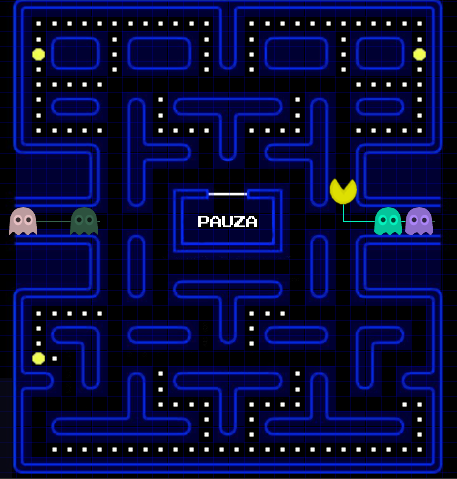
\includegraphics[width=13cm]{img/paclan1}
	\caption{Podział mapy na siatkę pól, zastosowanie heurystyki uwzględniającej zawijanie mapy po bokach, Źródło: własna implementacja gry}
	\label{fig:image_paclan1}
\end{figure}

\subsection{Metody zcentralizowane}
Wiele metod zcentralizowanych cechuje się planowaniem w zbiorowej przestrzeni konfiguracyjnej oraz możliwością wyznaczenia optymalnego rozwiązania.
Wadą jest natomiast duża złożoność obliczeniowa algorytmu i konieczność posiadania pełnej informacji o stanie otoczenia i robotów.

W systemach czasu rzeczywistego istotne jest, aby rozwiązanie problemu planowania tras uzyskać w określonym czasie, dlatego w tego typu sytemach częściej używane są techniki rozproszone.

$TODO$ Podejmowanie decyzji na podstawie centralnego systemu - scentralizowana struktura organizacyjna

\subsection{Metoda pól potencjałowych}
$TODO$ nie pisać, że to zcentralizowana, czy nie
Nie wszystkie podejścia zcentralizowane gwarantują optymalne rozwiązanie. Przykładem takiej metody, która nie daje gwarancji optymalności (ani nawet zupełności) jest metoda pól potencjałowych.

Metoda pól potencjałowych (ang. {\it Artificial Potential Field} lub {\it Potential Field Techniques}) polega na zastosowaniu zasad oddziaływania między ładunkami znanych z elektrostatyki. Roboty i przeszkody traktowane są jako ładunki jednoimienne, przez co "odpychają się" siłą odwrotnie proporcjonalną do kwadratu odległości (dzięki temu unikają kolizji między sobą). Natomiast punkt docelowy robota jest odwzorowany jako ładunek o przeciwnym biegunie, przez co robot jest "przyciągany" do celu.
Główną zasadę działania metody przedstawiono na rysunku \ref{fig:image_potentialfield}.
Technika ta jest bardzo prosta i nie wymaga wykonywania złożonych obliczeń (w odróżnieniu do pozostałych metod zcentralizowanych). Niestety bardzo powszechny jest problem osiągania minimum lokalnego, w którym suma wektorów daje zerową siłę wypadkową. Robot zostaje "uwięziony" w minimum lokalnym, przez co nie jest w stanie dotrzeć do wyznaczonego celu. Do omijania tego problemu muszą być stosowane inne dodatkowe metody. \cite{potentialfield}
\begin{figure}[H]
	\centering
	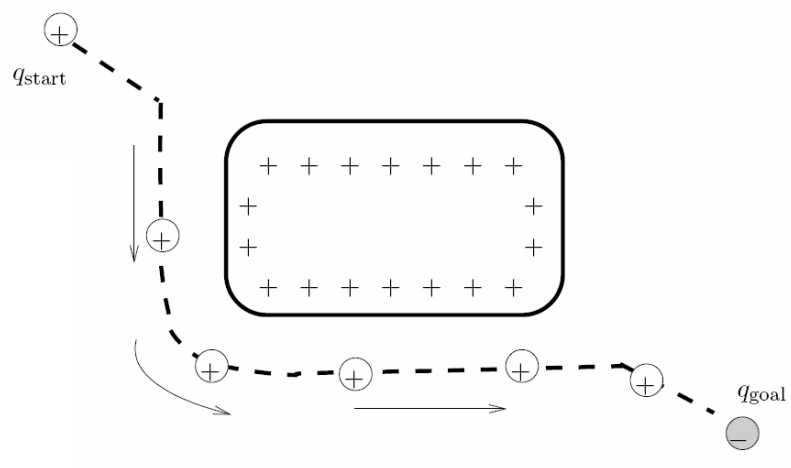
\includegraphics[width=12cm]{img/potential-field}
	\caption{Zasada działania metody pól potencjałowych. Źródło: \cite{howie_potentialfield}}
	\label{fig:image_potentialfield}
\end{figure}

\subsection{Rozproszone wyznaczanie tras}
$TODO$ wyjebać to gówno
Popularne podejścia unikające planowania w wysoko wymiarowej zbiorowej przestrzeni konfiguracyjnej to techniki rozproszone i priorytetowane.
Pomimo, że metody te są bardzo efektywne, mają dwie główne wady:
\begin{enumerate}
	\item Nie są zupełne - czasami nie udaje się znaleźć rozwiązania, nawet gdy istnieje.
	\item Wynikowe rozwiązania są często nieoptymalne.
\end{enumerate}

W artykule \cite{optpriorities} przedstawione zostało podejście do optymalizowania układu priorytetów dla rozproszonych i priorytetowanych technik planowania.
Proponowana metoda wykonuje randomizowane przeszukiwanie z techniką hill-climbing do znalezienia rozwiązania i do skrócenia całkowitej długości ścieżek.
Technika ta została zaimplemenotwana i przetestowana na prawdziwych robotach oraz w rozległych testach symulacyjnych.
Wyniki eksperyentu pokazały, że metoda potrafi znacząco zmniejszyć liczbę niepowodzeń i znacznie zmniejszyć całkowitą długość tras dla różnych priorytetowanych i rozproszoncyh metod planowania dróg, nawet dla dużych zespołów robotów.

Najczęściej stosowanymi podejściami są metody oparte o algorytm A*. W szczególności są to:
\begin{itemize}
	\item A* w konfiguracji czaso-przestrzennej
	\item Path coordination
\end{itemize}

\subsubsection{Path coordination}
Idea metody Path coordination przedstawia się następująco \cite{optpriorities}:
\begin{enumerate}
	\item Wyznaczenie ścieżki dla każdego robota {\bf niezależnie}
	\item Przydział priorytetów
	\item Próba rozwiązania możliwych konfliktów między ścieżkami. Roboty utrzymywane są na ich indywidualnych ścieżkach (wyznaczonych na początku), wprowadzane modyfikacje pozwalają na zatrzymanie się, ruch naprzód, a nawet cofanie się, ale tylko {\bf wzdłuż trajektorii} w celu uniknięcia kolizji z robotem o wyższym priorytecie.
\end{enumerate}
Złożoność metody wynosi $O(n \cdot m \cdot log(m))$, $m$ - maksymalna liczba stanów podczas planowania, $n$ - liczba robotów


\subsection{Priorytetowane planowanie}
$TODO$
In general, the complexity of complete approaches to multi-agent
path planning grows exponentially with the number of agents. There-
fore, the complete approaches often do not scale-up well and hence
are often not applicable for nontrivial domains with many agents. To
plan paths for a high number of agents in a complex environment,
one has to resort to one of the incomplete, but fast approaches. A
simple method often used in practice is prioritized planning [3, 9, 1].
In prioritized planning the agents are assigned a unique priority. In
its simplest form, the algorithm proceeds sequentially and agents
plan individually from the highest priority agent to the lowest one.
The agents consider the trajectories of higher priority agents as con-
straints (moving obstacles), which they need to avoid. It is straight-
forward to see that when the algorithm finishes, each agent is as-
signed a trajectory not colliding with either higher priority agents,
since the agent avoided a collision with those, nor with lower priority
agents who avoided a conflict with the given trajectory themselves.

The complexity of the generic algorithm grows linearly with the
number of agents, which makes the approach applicable for problems
involving many agents. Clearly, the algorithm is greedy and incom-
plete in the sense that agents are satisfied with the first trajectory not
colliding with higher priority agents and if a single agent is unable to
find a collision-free path for itself, the overall path finding algorithm
fails. The benefit, however, is fast runtime in relatively uncluttered
environments, which is often the case in multi-robotic applications.
Prioritized planner is also sensitive to the initial prioritization of the
agents. Both phenomena are illustrated in Figure 1 that shows a sim-
ple scenario with two agents desiring to move from s1 to d1 (s2 to d2
resp.) in a corridor that is only slightly wider than a single agent. The
scenario assumes that both agents have identical maximum speeds.
\cite{async_decentralized_spacetime_cp}


\begin{figure}[H]
	\centering
	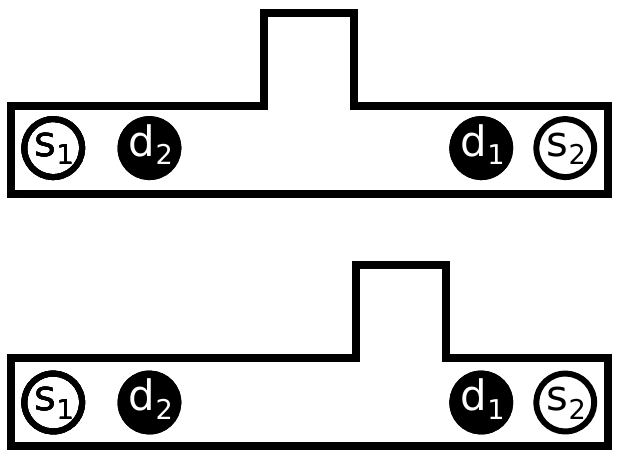
\includegraphics[width=10cm]{img/prioritized-planning-problem1}
	\caption{Top: example of a problem to which a prioritized planner
will not find a solution. The first agent plans its optimal path first,
but such a trajectory is in conflict with all feasible trajectories of the
second agent. Bottom: example of a problem to which a prioritized
planner will find a solution only if agent 1 has a higher priority than
agent 2. Źródło: \cite{async_decentralized_spacetime_cp}}
	\label{fig:img_prioritized-planning-problem1}
\end{figure}

\subsection{Wybór priorytetów}
$TODO$ nie dotyczy tylko Path coordination, ale też A* time-space
Istotną rolę doboru priorytetów robotów w procesie planowania tras ukazuje prosty przykład przedstawiony na rysunku \ref{fig:image_article1_fig1}. Jeśli robot 1 (zmierzający z punktu S1 do G1) otrzyma wyższy priorytet niż robot 2 (zmierzający z S2 do G2), spowoduje to zablokowanie przejazdu dla robota 2 i w efekcie prawidłowe rozwiązanie nie zostanie znalezione.
\begin{figure}[H]
	\centering
	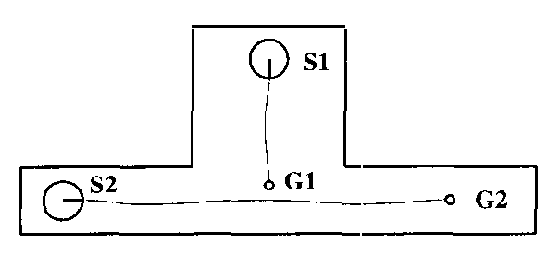
\includegraphics[width=10cm]{img/article1/fig1}
	\caption{Sytuacja, w której żadne rozwiązanie nie zostanie znalezione, jeśli robot 1 ma wyższy priorytet niż robot 2. Źródło: \cite{optpriorities}}
	\label{fig:image_article1_fig1}
\end{figure}

Układ priorytetów może mieć również zasadniczy wpływ na długość uzyskanych tras. Odpowiedni przykład został przedstawiony na rysunku \ref{fig:image_article1_ppt6}. W zależności od wyboru priorytetów, wpływających na kolejność planowania tras, otrzymujemy różne rozwiązania.
\begin{figure}[H]
	\centering
	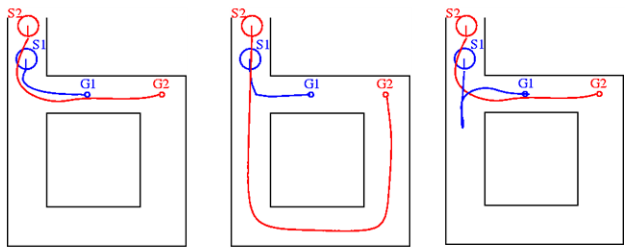
\includegraphics[width=13cm]{img/article1/ppt6}
	\caption{a) Niezależne planowanie optymalnych tras dla 2 robotów; b) suboptymalne rozwiązanie, gdy robot 1 ma wyższy priorytet; c) rozwiązanie, gdy robot 2 ma wyższy priorytet}
	\label{fig:image_article1_ppt6}
\end{figure}

\clearpage{\pagestyle{empty}\cleardoublepage}

\chapter{Podsumowanie}
\label{ch:podsumowanie}

$TODO$
Większość algorytmów Cooperative Pathfinding opiera się o A*

Algorytmy wprowadzają ograniczenie (błędne założenie), że ruchy trwają tyle samo. Można robić inaczej: podzielić dyskretnie i zaznaczać zajętość pól w wielu kratkach - ale wtedy będzie więcej obliczeń.

Windowed Hierarchical Cooperative A*:
• Cooperative A*
• Hierarchical Heuristic
• Windowed cooperation

The cooperative pathfinding methods are more successful
and find higher quality routes than A* with Local Repair.
Unfortunately, the basic CA* algorithm is costly to compute,

The size of the window has a significant effect on the suc-
cess and performance of the algorithm. With a large win-
dow, WHCA* behaves more like HCA* and the initialisa-
tion time increases. If the window is small, WHCA* be-
haves more like Local Repair A*. The success rate goes
down and the path length increases. The window size pa-
rameter thus provides a spectrum between Local Repair A*
and HCA*. An intermediate choice appears to give the most robust overall performance.
In general, the window size should be set to the duration
of the longest predicted bottleneck. In Real-Time Strategy
games groups of units are often moved together towards a
common destination. In this case the maximum bottleneck
time with cooperative pathfinding (ignoring units in other
groups) is the number of units in the group. If the window
size is lower than this threshold, bottleneck situations may
not be resolved well. If the window size is higher, then some
redundant search will be performed.

Local Repair A* may be an adequate solution for simple en-
vironments with few bottlenecks and few agents. With more
difficult environments, Local Repair A* is inadequate and is
significantly outperformed by Cooperative A* algorithms.

By introducing Hierarchical A* to improve the heuristic and
using windowing to shorten the search, a robust and efficient
algorithm, WHCA*, was developed. WHCA* finds more
successful routes than Local Repair A*, with shorter paths
and fewer cycles.

Although this research was restricted to grid environ-
ments, the algorithms presented here apply equally to more
general pathfinding domains. Any continuous environment
or navigational mesh can be used, so long as each agent’s
route can be planned by discrete motion elements. The grid-
based reservation table is generally applicable, but reserving
mesh intersections may be more appropriate in some cases.
Finally, the cooperative algorithms may be applied in dy-
namic environments, so long as an agent’s route is recom-
puted whenever invalidated by a change to the map.


Cooperative pathfinding is a general technique for coordinating the paths of many units.
It is appropriate whenever there are many units on the same side who are able to
communicate their paths. By planning ahead in time as well as space, units can get out of
each other’s way and avoid any conflicting routes.

Many of the usual enhancements to spatial A* can also be applied to space-time A*.
Moreover, the time dimension gives a whole new set of opportunities for pathfinding
algorithms to explore.

\clearpage{\pagestyle{empty}\cleardoublepage}

\phantomsection
\addcontentsline{toc}{chapter}{Bibliografia}
\bibliographystyle{unsrt}	
\bibliography{bibliography}
\clearpage

\phantomsection
\addcontentsline{toc}{chapter}{Wykaz skrótów}
\chapter*{Wykaz skrótów}

\begin{tabular}{l l}
API & Application Programming Interface \\
SDK & Software Development Kit \\


\end{tabular}


\phantomsection
\addcontentsline{toc}{chapter}{Spis rysunków}
\listoffigures

\phantomsection
\addcontentsline{toc}{chapter}{Spis tabel}
\listoftables